
% Default to the notebook output style

    


% Inherit from the specified cell style.




    
\documentclass[11pt,french]{article}

    
    \usepackage{babel}
    \usepackage[T1]{fontenc}
    % Nicer default font (+ math font) than Computer Modern for most use cases
    \usepackage{mathpazo}

    % Basic figure setup, for now with no caption control since it's done
    % automatically by Pandoc (which extracts ![](path) syntax from Markdown).
    \usepackage{graphicx}
    % We will generate all images so they have a width \maxwidth. This means
    % that they will get their normal width if they fit onto the page, but
    % are scaled down if they would overflow the margins.
    \makeatletter
    \def\maxwidth{\ifdim\Gin@nat@width>\linewidth\linewidth
    \else\Gin@nat@width\fi}
    \makeatother
    \let\Oldincludegraphics\includegraphics
    % Set max figure width to be 80% of text width, for now hardcoded.
    \renewcommand{\includegraphics}[1]{\Oldincludegraphics[width=.8\maxwidth]{#1}}
    % Ensure that by default, figures have no caption (until we provide a
    % proper Figure object with a Caption API and a way to capture that
    % in the conversion process - todo).
    \usepackage{caption}
    \DeclareCaptionLabelFormat{nolabel}{}
    \captionsetup{labelformat=nolabel}

    \usepackage{adjustbox} % Used to constrain images to a maximum size 
    \usepackage{xcolor} % Allow colors to be defined
    \usepackage{enumerate} % Needed for markdown enumerations to work
    \usepackage{geometry} % Used to adjust the document margins
    \usepackage{amsmath} % Equations
    \usepackage{amssymb} % Equations
    \usepackage{textcomp} % defines textquotesingle
    % Hack from http://tex.stackexchange.com/a/47451/13684:
    \AtBeginDocument{%
        \def\PYZsq{\textquotesingle}% Upright quotes in Pygmentized code
    }
    \usepackage{upquote} % Upright quotes for verbatim code
    \usepackage{eurosym} % defines \euro
    \usepackage[mathletters]{ucs} % Extended unicode (utf-8) support
    \usepackage[utf8x]{inputenc} % Allow utf-8 characters in the tex document
    \usepackage{fancyvrb} % verbatim replacement that allows latex
    \usepackage{grffile} % extends the file name processing of package graphics 
                         % to support a larger range 
    % The hyperref package gives us a pdf with properly built
    % internal navigation ('pdf bookmarks' for the table of contents,
    % internal cross-reference links, web links for URLs, etc.)
    \usepackage{hyperref}
    \usepackage{longtable} % longtable support required by pandoc >1.10
    \usepackage{booktabs}  % table support for pandoc > 1.12.2
    \usepackage[inline]{enumitem} % IRkernel/repr support (it uses the enumerate* environment)
    \usepackage[normalem]{ulem} % ulem is needed to support strikethroughs (\sout)
                                % normalem makes italics be italics, not underlines
    \usepackage{mathrsfs}
    

    
    
    % Colors for the hyperref package
    \definecolor{urlcolor}{rgb}{0,.145,.698}
    \definecolor{linkcolor}{rgb}{.71,0.21,0.01}
    \definecolor{citecolor}{rgb}{.12,.54,.11}

    % ANSI colors
    \definecolor{ansi-black}{HTML}{3E424D}
    \definecolor{ansi-black-intense}{HTML}{282C36}
    \definecolor{ansi-red}{HTML}{E75C58}
    \definecolor{ansi-red-intense}{HTML}{B22B31}
    \definecolor{ansi-green}{HTML}{00A250}
    \definecolor{ansi-green-intense}{HTML}{007427}
    \definecolor{ansi-yellow}{HTML}{DDB62B}
    \definecolor{ansi-yellow-intense}{HTML}{B27D12}
    \definecolor{ansi-blue}{HTML}{208FFB}
    \definecolor{ansi-blue-intense}{HTML}{0065CA}
    \definecolor{ansi-magenta}{HTML}{D160C4}
    \definecolor{ansi-magenta-intense}{HTML}{A03196}
    \definecolor{ansi-cyan}{HTML}{60C6C8}
    \definecolor{ansi-cyan-intense}{HTML}{258F8F}
    \definecolor{ansi-white}{HTML}{C5C1B4}
    \definecolor{ansi-white-intense}{HTML}{A1A6B2}
    \definecolor{ansi-default-inverse-fg}{HTML}{FFFFFF}
    \definecolor{ansi-default-inverse-bg}{HTML}{000000}

    % commands and environments needed by pandoc snippets
    % extracted from the output of `pandoc -s`
    \providecommand{\tightlist}{%
      \setlength{\itemsep}{0pt}\setlength{\parskip}{0pt}}
    \DefineVerbatimEnvironment{Highlighting}{Verbatim}{commandchars=\\\{\}}
    % Add ',fontsize=\small' for more characters per line
    \newenvironment{Shaded}{}{}
    \newcommand{\KeywordTok}[1]{\textcolor[rgb]{0.00,0.44,0.13}{\textbf{{#1}}}}
    \newcommand{\DataTypeTok}[1]{\textcolor[rgb]{0.56,0.13,0.00}{{#1}}}
    \newcommand{\DecValTok}[1]{\textcolor[rgb]{0.25,0.63,0.44}{{#1}}}
    \newcommand{\BaseNTok}[1]{\textcolor[rgb]{0.25,0.63,0.44}{{#1}}}
    \newcommand{\FloatTok}[1]{\textcolor[rgb]{0.25,0.63,0.44}{{#1}}}
    \newcommand{\CharTok}[1]{\textcolor[rgb]{0.25,0.44,0.63}{{#1}}}
    \newcommand{\StringTok}[1]{\textcolor[rgb]{0.25,0.44,0.63}{{#1}}}
    \newcommand{\CommentTok}[1]{\textcolor[rgb]{0.38,0.63,0.69}{\textit{{#1}}}}
    \newcommand{\OtherTok}[1]{\textcolor[rgb]{0.00,0.44,0.13}{{#1}}}
    \newcommand{\AlertTok}[1]{\textcolor[rgb]{1.00,0.00,0.00}{\textbf{{#1}}}}
    \newcommand{\FunctionTok}[1]{\textcolor[rgb]{0.02,0.16,0.49}{{#1}}}
    \newcommand{\RegionMarkerTok}[1]{{#1}}
    \newcommand{\ErrorTok}[1]{\textcolor[rgb]{1.00,0.00,0.00}{\textbf{{#1}}}}
    \newcommand{\NormalTok}[1]{{#1}}
    
    % Additional commands for more recent versions of Pandoc
    \newcommand{\ConstantTok}[1]{\textcolor[rgb]{0.53,0.00,0.00}{{#1}}}
    \newcommand{\SpecialCharTok}[1]{\textcolor[rgb]{0.25,0.44,0.63}{{#1}}}
    \newcommand{\VerbatimStringTok}[1]{\textcolor[rgb]{0.25,0.44,0.63}{{#1}}}
    \newcommand{\SpecialStringTok}[1]{\textcolor[rgb]{0.73,0.40,0.53}{{#1}}}
    \newcommand{\ImportTok}[1]{{#1}}
    \newcommand{\DocumentationTok}[1]{\textcolor[rgb]{0.73,0.13,0.13}{\textit{{#1}}}}
    \newcommand{\AnnotationTok}[1]{\textcolor[rgb]{0.38,0.63,0.69}{\textbf{\textit{{#1}}}}}
    \newcommand{\CommentVarTok}[1]{\textcolor[rgb]{0.38,0.63,0.69}{\textbf{\textit{{#1}}}}}
    \newcommand{\VariableTok}[1]{\textcolor[rgb]{0.10,0.09,0.49}{{#1}}}
    \newcommand{\ControlFlowTok}[1]{\textcolor[rgb]{0.00,0.44,0.13}{\textbf{{#1}}}}
    \newcommand{\OperatorTok}[1]{\textcolor[rgb]{0.40,0.40,0.40}{{#1}}}
    \newcommand{\BuiltInTok}[1]{{#1}}
    \newcommand{\ExtensionTok}[1]{{#1}}
    \newcommand{\PreprocessorTok}[1]{\textcolor[rgb]{0.74,0.48,0.00}{{#1}}}
    \newcommand{\AttributeTok}[1]{\textcolor[rgb]{0.49,0.56,0.16}{{#1}}}
    \newcommand{\InformationTok}[1]{\textcolor[rgb]{0.38,0.63,0.69}{\textbf{\textit{{#1}}}}}
    \newcommand{\WarningTok}[1]{\textcolor[rgb]{0.38,0.63,0.69}{\textbf{\textit{{#1}}}}}
    
    
    % Define a nice break command that doesn't care if a line doesn't already
    % exist.
    \def\br{\hspace*{\fill} \\* }
    % Math Jax compatibility definitions
    \def\gt{>}
    \def\lt{<}
    \let\Oldtex\TeX
    \let\Oldlatex\LaTeX
    \renewcommand{\TeX}{\textrm{\Oldtex}}
    \renewcommand{\LaTeX}{\textrm{\Oldlatex}}
    % Document parameters
    % Document title
    \title{Chap I Langage et constructions élémentaires}
    
    
    
    
    

    % Pygments definitions
    
\makeatletter
\def\PY@reset{\let\PY@it=\relax \let\PY@bf=\relax%
    \let\PY@ul=\relax \let\PY@tc=\relax%
    \let\PY@bc=\relax \let\PY@ff=\relax}
\def\PY@tok#1{\csname PY@tok@#1\endcsname}
\def\PY@toks#1+{\ifx\relax#1\empty\else%
    \PY@tok{#1}\expandafter\PY@toks\fi}
\def\PY@do#1{\PY@bc{\PY@tc{\PY@ul{%
    \PY@it{\PY@bf{\PY@ff{#1}}}}}}}
\def\PY#1#2{\PY@reset\PY@toks#1+\relax+\PY@do{#2}}

\expandafter\def\csname PY@tok@w\endcsname{\def\PY@tc##1{\textcolor[rgb]{0.73,0.73,0.73}{##1}}}
\expandafter\def\csname PY@tok@c\endcsname{\let\PY@it=\textit\def\PY@tc##1{\textcolor[rgb]{0.25,0.50,0.50}{##1}}}
\expandafter\def\csname PY@tok@cp\endcsname{\def\PY@tc##1{\textcolor[rgb]{0.74,0.48,0.00}{##1}}}
\expandafter\def\csname PY@tok@k\endcsname{\let\PY@bf=\textbf\def\PY@tc##1{\textcolor[rgb]{0.00,0.50,0.00}{##1}}}
\expandafter\def\csname PY@tok@kp\endcsname{\def\PY@tc##1{\textcolor[rgb]{0.00,0.50,0.00}{##1}}}
\expandafter\def\csname PY@tok@kt\endcsname{\def\PY@tc##1{\textcolor[rgb]{0.69,0.00,0.25}{##1}}}
\expandafter\def\csname PY@tok@o\endcsname{\def\PY@tc##1{\textcolor[rgb]{0.40,0.40,0.40}{##1}}}
\expandafter\def\csname PY@tok@ow\endcsname{\let\PY@bf=\textbf\def\PY@tc##1{\textcolor[rgb]{0.67,0.13,1.00}{##1}}}
\expandafter\def\csname PY@tok@nb\endcsname{\def\PY@tc##1{\textcolor[rgb]{0.00,0.50,0.00}{##1}}}
\expandafter\def\csname PY@tok@nf\endcsname{\def\PY@tc##1{\textcolor[rgb]{0.00,0.00,1.00}{##1}}}
\expandafter\def\csname PY@tok@nc\endcsname{\let\PY@bf=\textbf\def\PY@tc##1{\textcolor[rgb]{0.00,0.00,1.00}{##1}}}
\expandafter\def\csname PY@tok@nn\endcsname{\let\PY@bf=\textbf\def\PY@tc##1{\textcolor[rgb]{0.00,0.00,1.00}{##1}}}
\expandafter\def\csname PY@tok@ne\endcsname{\let\PY@bf=\textbf\def\PY@tc##1{\textcolor[rgb]{0.82,0.25,0.23}{##1}}}
\expandafter\def\csname PY@tok@nv\endcsname{\def\PY@tc##1{\textcolor[rgb]{0.10,0.09,0.49}{##1}}}
\expandafter\def\csname PY@tok@no\endcsname{\def\PY@tc##1{\textcolor[rgb]{0.53,0.00,0.00}{##1}}}
\expandafter\def\csname PY@tok@nl\endcsname{\def\PY@tc##1{\textcolor[rgb]{0.63,0.63,0.00}{##1}}}
\expandafter\def\csname PY@tok@ni\endcsname{\let\PY@bf=\textbf\def\PY@tc##1{\textcolor[rgb]{0.60,0.60,0.60}{##1}}}
\expandafter\def\csname PY@tok@na\endcsname{\def\PY@tc##1{\textcolor[rgb]{0.49,0.56,0.16}{##1}}}
\expandafter\def\csname PY@tok@nt\endcsname{\let\PY@bf=\textbf\def\PY@tc##1{\textcolor[rgb]{0.00,0.50,0.00}{##1}}}
\expandafter\def\csname PY@tok@nd\endcsname{\def\PY@tc##1{\textcolor[rgb]{0.67,0.13,1.00}{##1}}}
\expandafter\def\csname PY@tok@s\endcsname{\def\PY@tc##1{\textcolor[rgb]{0.73,0.13,0.13}{##1}}}
\expandafter\def\csname PY@tok@sd\endcsname{\let\PY@it=\textit\def\PY@tc##1{\textcolor[rgb]{0.73,0.13,0.13}{##1}}}
\expandafter\def\csname PY@tok@si\endcsname{\let\PY@bf=\textbf\def\PY@tc##1{\textcolor[rgb]{0.73,0.40,0.53}{##1}}}
\expandafter\def\csname PY@tok@se\endcsname{\let\PY@bf=\textbf\def\PY@tc##1{\textcolor[rgb]{0.73,0.40,0.13}{##1}}}
\expandafter\def\csname PY@tok@sr\endcsname{\def\PY@tc##1{\textcolor[rgb]{0.73,0.40,0.53}{##1}}}
\expandafter\def\csname PY@tok@ss\endcsname{\def\PY@tc##1{\textcolor[rgb]{0.10,0.09,0.49}{##1}}}
\expandafter\def\csname PY@tok@sx\endcsname{\def\PY@tc##1{\textcolor[rgb]{0.00,0.50,0.00}{##1}}}
\expandafter\def\csname PY@tok@m\endcsname{\def\PY@tc##1{\textcolor[rgb]{0.40,0.40,0.40}{##1}}}
\expandafter\def\csname PY@tok@gh\endcsname{\let\PY@bf=\textbf\def\PY@tc##1{\textcolor[rgb]{0.00,0.00,0.50}{##1}}}
\expandafter\def\csname PY@tok@gu\endcsname{\let\PY@bf=\textbf\def\PY@tc##1{\textcolor[rgb]{0.50,0.00,0.50}{##1}}}
\expandafter\def\csname PY@tok@gd\endcsname{\def\PY@tc##1{\textcolor[rgb]{0.63,0.00,0.00}{##1}}}
\expandafter\def\csname PY@tok@gi\endcsname{\def\PY@tc##1{\textcolor[rgb]{0.00,0.63,0.00}{##1}}}
\expandafter\def\csname PY@tok@gr\endcsname{\def\PY@tc##1{\textcolor[rgb]{1.00,0.00,0.00}{##1}}}
\expandafter\def\csname PY@tok@ge\endcsname{\let\PY@it=\textit}
\expandafter\def\csname PY@tok@gs\endcsname{\let\PY@bf=\textbf}
\expandafter\def\csname PY@tok@gp\endcsname{\let\PY@bf=\textbf\def\PY@tc##1{\textcolor[rgb]{0.00,0.00,0.50}{##1}}}
\expandafter\def\csname PY@tok@go\endcsname{\def\PY@tc##1{\textcolor[rgb]{0.53,0.53,0.53}{##1}}}
\expandafter\def\csname PY@tok@gt\endcsname{\def\PY@tc##1{\textcolor[rgb]{0.00,0.27,0.87}{##1}}}
\expandafter\def\csname PY@tok@err\endcsname{\def\PY@bc##1{\setlength{\fboxsep}{0pt}\fcolorbox[rgb]{1.00,0.00,0.00}{1,1,1}{\strut ##1}}}
\expandafter\def\csname PY@tok@kc\endcsname{\let\PY@bf=\textbf\def\PY@tc##1{\textcolor[rgb]{0.00,0.50,0.00}{##1}}}
\expandafter\def\csname PY@tok@kd\endcsname{\let\PY@bf=\textbf\def\PY@tc##1{\textcolor[rgb]{0.00,0.50,0.00}{##1}}}
\expandafter\def\csname PY@tok@kn\endcsname{\let\PY@bf=\textbf\def\PY@tc##1{\textcolor[rgb]{0.00,0.50,0.00}{##1}}}
\expandafter\def\csname PY@tok@kr\endcsname{\let\PY@bf=\textbf\def\PY@tc##1{\textcolor[rgb]{0.00,0.50,0.00}{##1}}}
\expandafter\def\csname PY@tok@bp\endcsname{\def\PY@tc##1{\textcolor[rgb]{0.00,0.50,0.00}{##1}}}
\expandafter\def\csname PY@tok@fm\endcsname{\def\PY@tc##1{\textcolor[rgb]{0.00,0.00,1.00}{##1}}}
\expandafter\def\csname PY@tok@vc\endcsname{\def\PY@tc##1{\textcolor[rgb]{0.10,0.09,0.49}{##1}}}
\expandafter\def\csname PY@tok@vg\endcsname{\def\PY@tc##1{\textcolor[rgb]{0.10,0.09,0.49}{##1}}}
\expandafter\def\csname PY@tok@vi\endcsname{\def\PY@tc##1{\textcolor[rgb]{0.10,0.09,0.49}{##1}}}
\expandafter\def\csname PY@tok@vm\endcsname{\def\PY@tc##1{\textcolor[rgb]{0.10,0.09,0.49}{##1}}}
\expandafter\def\csname PY@tok@sa\endcsname{\def\PY@tc##1{\textcolor[rgb]{0.73,0.13,0.13}{##1}}}
\expandafter\def\csname PY@tok@sb\endcsname{\def\PY@tc##1{\textcolor[rgb]{0.73,0.13,0.13}{##1}}}
\expandafter\def\csname PY@tok@sc\endcsname{\def\PY@tc##1{\textcolor[rgb]{0.73,0.13,0.13}{##1}}}
\expandafter\def\csname PY@tok@dl\endcsname{\def\PY@tc##1{\textcolor[rgb]{0.73,0.13,0.13}{##1}}}
\expandafter\def\csname PY@tok@s2\endcsname{\def\PY@tc##1{\textcolor[rgb]{0.73,0.13,0.13}{##1}}}
\expandafter\def\csname PY@tok@sh\endcsname{\def\PY@tc##1{\textcolor[rgb]{0.73,0.13,0.13}{##1}}}
\expandafter\def\csname PY@tok@s1\endcsname{\def\PY@tc##1{\textcolor[rgb]{0.73,0.13,0.13}{##1}}}
\expandafter\def\csname PY@tok@mb\endcsname{\def\PY@tc##1{\textcolor[rgb]{0.40,0.40,0.40}{##1}}}
\expandafter\def\csname PY@tok@mf\endcsname{\def\PY@tc##1{\textcolor[rgb]{0.40,0.40,0.40}{##1}}}
\expandafter\def\csname PY@tok@mh\endcsname{\def\PY@tc##1{\textcolor[rgb]{0.40,0.40,0.40}{##1}}}
\expandafter\def\csname PY@tok@mi\endcsname{\def\PY@tc##1{\textcolor[rgb]{0.40,0.40,0.40}{##1}}}
\expandafter\def\csname PY@tok@il\endcsname{\def\PY@tc##1{\textcolor[rgb]{0.40,0.40,0.40}{##1}}}
\expandafter\def\csname PY@tok@mo\endcsname{\def\PY@tc##1{\textcolor[rgb]{0.40,0.40,0.40}{##1}}}
\expandafter\def\csname PY@tok@ch\endcsname{\let\PY@it=\textit\def\PY@tc##1{\textcolor[rgb]{0.25,0.50,0.50}{##1}}}
\expandafter\def\csname PY@tok@cm\endcsname{\let\PY@it=\textit\def\PY@tc##1{\textcolor[rgb]{0.25,0.50,0.50}{##1}}}
\expandafter\def\csname PY@tok@cpf\endcsname{\let\PY@it=\textit\def\PY@tc##1{\textcolor[rgb]{0.25,0.50,0.50}{##1}}}
\expandafter\def\csname PY@tok@c1\endcsname{\let\PY@it=\textit\def\PY@tc##1{\textcolor[rgb]{0.25,0.50,0.50}{##1}}}
\expandafter\def\csname PY@tok@cs\endcsname{\let\PY@it=\textit\def\PY@tc##1{\textcolor[rgb]{0.25,0.50,0.50}{##1}}}

\def\PYZbs{\char`\\}
\def\PYZus{\char`\_}
\def\PYZob{\char`\{}
\def\PYZcb{\char`\}}
\def\PYZca{\char`\^}
\def\PYZam{\char`\&}
\def\PYZlt{\char`\<}
\def\PYZgt{\char`\>}
\def\PYZsh{\char`\#}
\def\PYZpc{\char`\%}
\def\PYZdl{\char`\$}
\def\PYZhy{\char`\-}
\def\PYZsq{\char`\'}
\def\PYZdq{\char`\"}
\def\PYZti{\char`\~}
% for compatibility with earlier versions
\def\PYZat{@}
\def\PYZlb{[}
\def\PYZrb{]}
\makeatother


    % Exact colors from NB
    \definecolor{incolor}{rgb}{0.0, 0.0, 0.5}
    \definecolor{outcolor}{rgb}{0.545, 0.0, 0.0}



    
    % Prevent overflowing lines due to hard-to-break entities
    \sloppy 
    % Setup hyperref package
    \hypersetup{
      breaklinks=true,  % so long urls are correctly broken across lines
      colorlinks=true,
      urlcolor=urlcolor,
      linkcolor=linkcolor,
      citecolor=citecolor,
      }
    % Slightly bigger margins than the latex defaults
    
    \geometry{verbose,tmargin=1in,bmargin=1in,lmargin=1in,rmargin=1in}
    
    
	\author{\textsc{Bruno Darid}}
    \begin{document}
    \renewcommand{\contentsname}{\textsc{Plan}}    
 	\maketitle
 	\tableofcontents
 

    \hypertarget{repuxe8res-historiques}{%
\section{Repères historiques}\label{repuxe8res-historiques}}

\begin{figure}[h]
	\begin{center}
		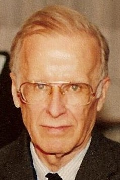
\includegraphics{John_Backus_3.png}
	\end{center}
	\caption{Fig. \ref{fig:backus} -- John Backus}
	\label{fig:backus}
\end{figure}

En 1954, \href{https://fr.wikipedia.org/wiki/John_Backus}{John
Backus}(\emph{1924-2007}), fig. \ref{fig:backus}, présente le premier vrai langage de
programmation tel qu'on l'entend aujourd'hui: le
\href{https://fr.wikipedia.org/wiki/Fortran}{Fortran}. Il mit au point
vers la fin des années 50 le langage
\href{https://fr.wikipedia.org/wiki/Algol_(langage)}{Algol}. Il a, par
la suite, proposé la \emph{forme Backus-Naur}, notation qui permet de
décrire la \emph{grammaire} des langages de programmation.

    \hypertarget{le-langage-python}{%
\section{Le langage Python}\label{le-langage-python}}

 \hypertarget{intro}{%
\subsection{Introduction}\label{intro}}

  Un programme est un texte qui décrit un algorithme que l'on souhaite
  faire exécuter par une machine. Ce texte est écrit dans un langage
  particulier, appelé \textbf{langage de programmation}. Le premier
  langage abordé en spécialité NSI est le langage \textbf{Python} en
  version 3. C'est un langage de haut niveau (\emph{d'abstraction}) et
  interprété (\emph{un programme appelé interpréteur se charge
  d'exécuter ligne par ligne le code \og source\fg}).

  \hypertarget{io}{%
\subsection{Les entrées/sorties}\label{io}}
  Dans un langage de programmation on appelle \textbf{entrées/sorties} des
  constructions permettant une communication avec l'utilisateur, donnant
  ainsi un aspect interactif au programme.\par
  En python l'instruction \texttt{print()} affiche à l'écran les
  objets passés en arguments. Dans les exemples qui vont suivre, on affiche des chaînes de caractères (en python ces dernières sont délimitées par des doubles quotes \texttt{" "} ou des simples quotes \texttt{' '}).


    \begin{Verbatim}[commandchars=\\\{\}]
{\color{incolor}In [{\color{incolor} }]:} \PY{n+nb}{print}\PY{p}{(}\PY{l+s+s2}{\PYZdq{}}\PY{l+s+s2}{Hello World!}\PY{l+s+s2}{\PYZdq{}}\PY{p}{)}
        \PY{n+nb}{print}\PY{p}{(}\PY{l+s+s2}{\PYZdq{}}\PY{l+s+s2}{Python version 3.}\PY{l+s+s2}{\PYZdq{}}\PY{p}{,} \PY{l+s+s2}{\PYZdq{}}\PY{l+s+s2}{Environnement}\PY{l+s+s2}{\PYZdq{}}\PY{p}{,} \PY{l+s+s2}{\PYZdq{}}\PY{l+s+s2}{Jupyter Notebook 5.7}\PY{l+s+s2}{\PYZdq{}}\PY{p}{)}
        \PY{n+nb}{print}\PY{p}{(}\PY{l+s+s2}{\PYZdq{}}\PY{l+s+s2}{Python version 3.}\PY{l+s+s2}{\PYZdq{}}\PY{p}{,} \PY{l+s+s2}{\PYZdq{}}\PY{l+s+s2}{Env.}\PY{l+s+s2}{\PYZdq{}}\PY{p}{,} \PY{l+s+s2}{\PYZdq{}}\PY{l+s+s2}{Jupyter}\PY{l+s+s2}{\PYZdq{}}\PY{p}{,} \PY{n}{sep}\PY{o}{=}\PY{l+s+s2}{\PYZdq{}}\PY{l+s+s2}{//}\PY{l+s+s2}{\PYZdq{}}\PY{p}{,} \PY{n}{end}\PY{o}{=}\PY{l+s+s2}{\PYZdq{}}\PY{l+s+s2}{ }\PY{l+s+s2}{\PYZdq{}}\PY{p}{)}
        \PY{n+nb}{print}\PY{p}{(}\PY{l+s+s2}{\PYZdq{}}\PY{l+s+s2}{Pas de retour à la ligne.}\PY{l+s+s2}{\PYZdq{}}\PY{p}{)}
\end{Verbatim}

    Des arguments optionnels comme \texttt{sep} ou \texttt{end} par exemple,
permettent d'adapter l'affichage aux besoins.
Par ailleurs, l'instruction \texttt{input()} interrompt le déroulement
du programme et attend que l'utilisateur tape quelque chose au clavier.

    \begin{Verbatim}[commandchars=\\\{\}]
{\color{incolor}In [{\color{incolor} }]:} \PY{n}{niveau} \PY{o}{=} \PY{n+nb}{input}\PY{p}{(}\PY{l+s+s2}{\PYZdq{}}\PY{l+s+s2}{Quel est votre niveau (novice/intermédiaire/avancé)?}\PY{l+s+s2}{\PYZdq{}}\PY{p}{)}
        \PY{n}{moyenne} \PY{o}{=} \PY{n+nb}{input}\PY{p}{(}\PY{l+s+s2}{\PYZdq{}}\PY{l+s+s2}{Quelle était votre moyenne annuelle en math ?}\PY{l+s+s2}{\PYZdq{}}\PY{p}{)}
        \PY{n+nb}{print}\PY{p}{(}\PY{l+s+s2}{\PYZdq{}}\PY{l+s+s2}{Vous avez répondu:}\PY{l+s+s2}{\PYZdq{}}\PY{p}{,}\PY{n}{niveau}\PY{p}{,}\PY{l+s+s2}{\PYZdq{}}\PY{l+s+s2}{avec }\PY{l+s+s2}{\PYZdq{}}\PY{p}{,} \PY{n}{moyenne}\PY{p}{,} \PY{l+s+s2}{\PYZdq{}}\PY{l+s+s2}{en math!}\PY{l+s+s2}{\PYZdq{}}\PY{p}{)}
\end{Verbatim}

    \emph{Remarques}
    \begin{itemize}
	\item \texttt{input()} retourne toujours une chaine de caractères (même si
	l'utilisateur entre un nombre!);
	\item  la syntaxe employée à l'intérieur de la fonction \texttt{print()} bien
que correcte, sera simplifiée dans les cours ultérieurs tenant compte
des dernières évolutions du langage.
	\end{itemize}

\hypertarget{les-instructions-simples}{%
\section{Les instructions simples}\label{les-instructions-simples}}

Pour pouvoir accéder aux données, un programme d'ordinateur fait
abondamment usage de \textbf{variables}. Une variable est une
\emph{référence} désignant une \textbf{adresse mémoire}, c'est-à-dire un
emplacement précis dans la mémoire vive.\par
Les instructions \emph{simples} sont la \textbf{déclaration et
l'affectation de variables}. En python cette opération est réalisée de
la manière suivante:
\texttt{nom\_variable\ =\ valeur}. Par exemple
\begin{Shaded}
\begin{Highlighting}[]
\NormalTok{n }\OperatorTok{=} \DecValTok{7}
\NormalTok{msg }\OperatorTok{=} \StringTok{"Affectation"}
\NormalTok{pi }\OperatorTok{=} \FloatTok{3.14}
\end{Highlighting}
\end{Shaded}

\emph{Remarques}
\begin{itemize}
\item Le nom de variable doit commencer par une lettre et ne pas être un mot
réservé (voir
\href{https://docs.python.org/fr/3.7/reference/lexical_analysis.html\#keywords}{liste});
\item Contrairement à d'autres langages, on n'indique pas le type d'une
variable lors de sa déclaration en python. Le type est déterminé lors de
l'affectation. Dans l'exemple précédent, \texttt{n} est du type entier,
\texttt{msg} est du type chaîne de caractères, \texttt{pi} est du type
\emph{flottant} (décimal).
\end{itemize}

    \hypertarget{les-instructions-composuxe9es}{%
\section{Les instructions
composées}\label{les-instructions-composuxe9es}}

\hypertarget{la-suxe9quence}{%
\subsection{La séquence}\label{la-suxe9quence}}

On peut définir une séquence d'instruction comme un ensemble de deux
instructions exécutées l'une \textbf{à la suite} de l'autre (l'ordre est
important!). Par exemple, les lignes

\begin{Shaded}
\begin{Highlighting}[]
	\NormalTok{x }\OperatorTok{=}\NormalTok{ x }\OperatorTok{+} \DecValTok{1}
	\NormalTok{x }\OperatorTok{=}\NormalTok{ x }\OperatorTok{*} \DecValTok{2}
\end{Highlighting}
\end{Shaded}

constituent une séquence d'instructions (\emph{à condition que la
variable x ait été affectée au préalable!}). Nos programmes comporteront
généralement des séquences de plus de deux instructions, on parlera
alors de \textbf{bloc d'instructions}.

\textbf{Exercice E1C1}

Soit un disque de centre O et de rayon \(r\). \'Ecrire un programme qui
calcule et affiche l'aire \(S\) de ce disque à partir de la valeur du
rayon qui sera demandée à l'utilisateur. \emph{Indication}:
\(S=\pi*r^{2}\).

    \begin{Verbatim}[commandchars=\\\{\}]
{\color{incolor}In [{\color{incolor}23}]:} \PY{n}{pi} \PY{o}{=} \PY{l+m+mf}{3.14}
         \PY{c+c1}{\PYZsh{}Code à rajouter au dessous.}
         \PY{c+c1}{\PYZsh{}Toute suite de caractères (jusqu\PYZsq{}à la fin de ligne) placés après un}
         \PY{c+c1}{\PYZsh{}dièse est ignorée.On s\PYZsq{}en sert pour placer des commentaires.}
\end{Verbatim}

    \hypertarget{le-test}{%
\subsection{Le test}\label{le-test}}

\hypertarget{le-test-simple} désigne le reste de la division
euclidienne et \texttt{==} désigne l'égalité au sens test (et non
l'affectation!)

    \begin{Verbatim}[commandchars=\\\{\}]
{\color{incolor}In [{\color{incolor}1}]:} \PY{n}{x} \PY{o}{=} \PY{n+nb}{int}\PY{p}{(}\PY{n+nb}{input}\PY{p}{(}\PY{l+s+s2}{\PYZdq{}}\PY{l+s+s2}{Entrer un nombre: }\PY{l+s+s2}{\PYZdq{}}\PY{p}{)}\PY{p}{)}\PY{c+c1}{\PYZsh{} \PYZsq{}int\PYZsq{} convertit l'entrée en entier}
        \PY{k}{if} \PY{n}{x}\PY{o}{\PYZpc{}}\PY{k}{2} == 0:\PYZsh{}Si le reste de la division de x par 2 est nul
            \PY{n+nb}{print}\PY{p}{(}\PY{l+s+s2}{\PYZdq{}}\PY{l+s+s2}{Le reste de sa division par 2 est nul, }\PY{l+s+s2}{\PYZdq{}}\PY{p}{)}
            \PY{n+nb}{print}\PY{p}{(}\PY{n}{x}\PY{p}{,}\PY{l+s+s2}{\PYZdq{}}\PY{l+s+s2}{est un nombre pair.}\PY{l+s+s2}{\PYZdq{}}\PY{p}{)}\PY{c+c1}{\PYZsh{}alors on affiche la parité}
\end{Verbatim}

    \begin{Verbatim}[commandchars=\\\{\}]
Entrer un nombre: 6
Le reste de sa division par 2 est nul, 
6 est un nombre pair.

    \end{Verbatim}

    Pour identifier sans ambiguités les instructions appartenant au bloc
vérifiant la condition, on \textbf{DOIT LES INDENTER} en python.
Indenter signifie décaler d'un certain nombre de colonne (\emph{la bonne
pratique indique 4 espaces}) par rapport au bloc d'instructions
précédent.\\
La condition est souvent exprimée avec des opérateurs de comparaisons,
dont voici la liste:

\begin{Shaded}
\begin{Highlighting}[]
\NormalTok{x }\OperatorTok{==}\NormalTok{ y }\CommentTok{# x est égal à y}
\NormalTok{x }\OperatorTok{!=}\NormalTok{ y }\CommentTok{# x est différent de y}
\NormalTok{x }\OperatorTok{>}\NormalTok{ y }\CommentTok{# x est plus grand que y}
\NormalTok{x }\OperatorTok{<}\NormalTok{ y }\CommentTok{# x est plus petit que y}
\NormalTok{x }\OperatorTok{>=}\NormalTok{ y }\CommentTok{# x est plus grand que, ou égal à y}
\NormalTok{x }\OperatorTok{<=}\NormalTok{ y }\CommentTok{# x est plus petit que, ou égal à y}
\end{Highlighting}
\end{Shaded}

\noindent\textbf{Exercice E2C1: nombre pair divisible par 8}\\
\'Ecrire un programme python qui affiche le message ``N est pair et
divisible par 8'' si le nombre \(N\) demandé à l'utilisateur vérifie
cette condition.\\
\textbf{Exercice E3C1: valeur absolue}\\
\'Ecrire un programme qui transforme un nombre demandé à l'utilisateur, en
sa valeur absolue. 

\hypertarget{le-test-alternative}{%
\subsubsection{Le test avec alternative}\label{le-test-alternative}}
Parfois il est intéressant d'indiquer un bloc à traiter lorsque la condition
\emph{n'est pas} vérifiée. La syntaxe devient alors:

\begin{Shaded}
\begin{Highlighting}[]
\ControlFlowTok{if}\NormalTok{ condition:}
\NormalTok{    bloc_instructions_SI}
\ControlFlowTok{else}\NormalTok{:}
\NormalTok{    bloc_instructions_SINON}
\end{Highlighting}
\end{Shaded}

L'exemple précédent devient:

    \begin{Verbatim}[commandchars=\\\{\}]
{\color{incolor}In [{\color{incolor}2}]:} \PY{n}{x} \PY{o}{=} \PY{n+nb}{int}\PY{p}{(}\PY{n+nb}{input}\PY{p}{(}\PY{l+s+s2}{\PYZdq{}}\PY{l+s+s2}{Entrer un nombre: }\PY{l+s+s2}{\PYZdq{}}\PY{p}{)}\PY{p}{)}\PY{c+c1}{\PYZsh{} \PYZsq{}int\PYZsq{} convertit l'entrée en entier}
        \PY{k}{if} \PY{n}{x}\PY{o}{\PYZpc{}}\PY{k}{2} == 0:\PYZsh{}Si le reste de la division de x par 2 est nul
            \PY{n+nb}{print}\PY{p}{(}\PY{l+s+s2}{\PYZdq{}}\PY{l+s+s2}{Le reste de sa division par 2 est nul, }\PY{l+s+s2}{\PYZdq{}}\PY{p}{)}
            \PY{n+nb}{print}\PY{p}{(}\PY{n}{x}\PY{p}{,}\PY{l+s+s2}{\PYZdq{}}\PY{l+s+s2}{est un nombre pair.}\PY{l+s+s2}{\PYZdq{}}\PY{p}{)}\PY{c+c1}{\PYZsh{}alors on affiche la parité}
        \PY{k}{else}\PY{p}{:}\PY{c+c1}{\PYZsh{}x\PYZpc{}2 est donc différent de 0}
            \PY{n+nb}{print}\PY{p}{(}\PY{l+s+s2}{\PYZdq{}}\PY{l+s+s2}{Le reste de sa division par 2 n}\PY{l+s+s2}{\PYZsq{}}\PY{l+s+s2}{est pas nul, }\PY{l+s+s2}{\PYZdq{}}\PY{p}{)}
            \PY{n+nb}{print}\PY{p}{(}\PY{n}{x}\PY{p}{,}\PY{l+s+s2}{\PYZdq{}}\PY{l+s+s2}{est un nombre impair.}\PY{l+s+s2}{\PYZdq{}}\PY{p}{)}
\end{Verbatim}

    \begin{Verbatim}[commandchars=\\\{\}]
Entrer un nombre: 57
Le reste de sa division par 2 n'est pas nul, 
57 est un nombre impair.
    \end{Verbatim}

    Question: aurait-on pu utiliser le code suivant pour tester la parité
d'un nombre?

\begin{Shaded}
\begin{Highlighting}[]
\NormalTok{x }\OperatorTok{=} \BuiltInTok{int}\NormalTok{(}\BuiltInTok{input}\NormalTok{(}\StringTok{"Entrer un nombre: "}\NormalTok{))}\CommentTok{#int sert à convertir notre entrée en entier}
\ControlFlowTok{if}\NormalTok{ x}\OperatorTok{%}\DecValTok{2} \OperatorTok{==} \DecValTok{0}\NormalTok{:}\CommentTok{#Si le reste de la division de x par 2 est nul}
    \BuiltInTok{print}\NormalTok{(}\StringTok{"Le reste de sa division par 2 est nul, "}\NormalTok{)}
    \BuiltInTok{print}\NormalTok{(x,}\StringTok{"est un nombre pair."}\NormalTok{)}\CommentTok{#alors on affiche la parité}
    \ControlFlowTok{else}\NormalTok{:}\CommentTok{#x%2 est donc différent de 0}
        \BuiltInTok{print}\NormalTok{(}\StringTok{"Le reste de sa division par 2 n'est pas nul, "}\NormalTok{)}
        \BuiltInTok{print}\NormalTok{(x,}\StringTok{"est un nombre impair."}\NormalTok{)}
\end{Highlighting}
\end{Shaded}

 \textbf{Exercice E4C1: Que doit-on emmener?}\\
\'Ecrire un programme capable de conseiller deux objets utiles à emporter
en voyage, en fonction de la température de l'air. On demande à
l'utilisateur la température prévue. Si celle-ci est supérieure à 20°,
il conseille ``maillot'' et ``crème bronzante''. Sinon, il conseille
``parapluie'' et ``pull''.

 \textbf{Exercice E5C1: année bissextile}\\
Une année est bissextile si son millésime est multiple de 4. Cependant,
les années dont le millésime est multiple de 100 ne sont bissextiles que
si c'est aussi un multiple de 400 (\emph{1900 n'était pas bissextile,
2000 l'a été}). \'Ecrire un programme qui détermine si une année \(N\) est
bissextile ou non.\\
\href{./images/bissext.png}{Coup de pouce ?}

\textbf{Problème P1C1: Affichage de l'heure}\\
\'Ecrire un programme qui récupère l'heure d'un utilisateur sous la forme
HH mm ss. Le programme doit afficher cette heure augmentée d'une
seconde.

    \hypertarget{la-boucle}{%
\subsection{La boucle}\label{la-boucle}}

\hypertarget{la-boucle-conditionnelle-non-bornuxe9e}{%
\subsubsection{\texorpdfstring{La boucle conditionnelle, \emph{non
bornée}}{La boucle conditionnelle, non bornée}}\label{la-boucle-conditionnelle-non-bornuxe9e}}

\hypertarget{nuxe9cessituxe9}{%
\paragraph{Nécessité}\label{nuxe9cessituxe9}}

\begin{enumerate}
\def\labelenumi{\arabic{enumi}.}
\tightlist
\item
  Exécuter le programme ci-dessous pour des valeurs de \(N\) entières
  comprises entre 1 et 4. Que réalise-t-il?
\item
  Quel commentaire peut-on faire à propos du bloc d'instruction
  conditionnel?
\item
  Que faudrait-il apporter comme modification (\emph{ne pas le faire!})
  si on souhaitait rendre possible le calcul jusqu'à \(N=10\)?
\end{enumerate}

    \begin{Verbatim}[commandchars=\\\{\}]
{\color{incolor}In [{\color{incolor}7}]:} \PY{n}{N} \PY{o}{=} \PY{l+m+mi}{4}
        \PY{n}{c} \PY{o}{=} \PY{n}{N}
        \PY{n}{p} \PY{o}{=} \PY{l+m+mi}{1}
        \PY{k}{if} \PY{n}{c} \PY{o}{!=} \PY{l+m+mi}{0}\PY{p}{:}
            \PY{n}{p} \PY{o}{=} \PY{n}{p} \PY{o}{*} \PY{l+m+mi}{2}
            \PY{n}{c} \PY{o}{=} \PY{n}{c} \PY{o}{\PYZhy{}} \PY{l+m+mi}{1}
            \PY{k}{if} \PY{n}{c} \PY{o}{!=} \PY{l+m+mi}{0}\PY{p}{:}
                \PY{n}{p} \PY{o}{=} \PY{n}{p} \PY{o}{*} \PY{l+m+mi}{2}
                \PY{n}{c} \PY{o}{=} \PY{n}{c} \PY{o}{\PYZhy{}} \PY{l+m+mi}{1}
                \PY{k}{if} \PY{n}{c} \PY{o}{!=} \PY{l+m+mi}{0}\PY{p}{:}
                    \PY{n}{p} \PY{o}{=} \PY{n}{p} \PY{o}{*} \PY{l+m+mi}{2}
                    \PY{n}{c} \PY{o}{=} \PY{n}{c} \PY{o}{\PYZhy{}} \PY{l+m+mi}{1}
                    \PY{k}{if} \PY{n}{c} \PY{o}{!=} \PY{l+m+mi}{0}\PY{p}{:}
                        \PY{n}{p} \PY{o}{=} \PY{n}{p} \PY{o}{*} \PY{l+m+mi}{2}
                        \PY{n}{c} \PY{o}{=} \PY{n}{c} \PY{o}{\PYZhy{}} \PY{l+m+mi}{1}
        \PY{n+nb}{print}\PY{p}{(}\PY{n}{p}\PY{p}{)}
\end{Verbatim}
    \begin{Verbatim}[commandchars=\\\{\}]
16
    \end{Verbatim}

    La méthode précédente montre ses limites: pour des valeurs quelconques
de \(N\) il faudrait répéter un grand nombre de fois les mêmes lignes.
On aimerait exécuter les instructions

\begin{Shaded}
\begin{Highlighting}[]
\NormalTok{p }\OperatorTok{=}\NormalTok{ p }\OperatorTok{*} \DecValTok{2}
\NormalTok{c }\OperatorTok{=}\NormalTok{ c }\OperatorTok{-} \DecValTok{1}
\end{Highlighting}
\end{Shaded}

tant que le test \texttt{c\ !=\ 0} est vérifié. Il s'agit d'une
\textbf{boucle conditionnelle} ou encore \textbf{boucle while} (\emph{en
anglais}) ou \textbf{boucle tant que} (\emph{en français}).

    \hypertarget{syntaxe}{%
\subsubsection{Syntaxe}\label{syntaxe}}
En python, la boucle conditionnelle a la forme
suivante:

\begin{Shaded}
\begin{Highlighting}[]
\ControlFlowTok{while}\NormalTok{ condition:}
\NormalTok{    bloc_instructions}
\end{Highlighting}
\end{Shaded}

\emph{Remarques}
\begin{itemize}
\item la condition s'exprime souvent avec les opérateurs de comparaisons vu
plus haut;
\item le bloc d'instructions est indenté.
\end{itemize}
Le programme précédent peut ainsi s'écrire (\emph{le vérifier en l'exécutant}):

    \begin{Verbatim}[commandchars=\\\{\}]
{\color{incolor}In [{\color{incolor}18}]:} \PY{n}{N} \PY{o}{=} \PY{l+m+mi}{8}
         \PY{n}{c} \PY{o}{=} \PY{n}{N}
         \PY{n}{p} \PY{o}{=} \PY{l+m+mi}{1}
         \PY{k}{while} \PY{n}{c} \PY{o}{\PYZgt{}} \PY{l+m+mi}{0}\PY{p}{:}
             \PY{n}{p} \PY{o}{=} \PY{n}{p} \PY{o}{*} \PY{l+m+mi}{2}
             \PY{n}{c} \PY{o}{=} \PY{n}{c} \PY{o}{\PYZhy{}} \PY{l+m+mi}{1}
         \PY{n+nb}{print}\PY{p}{(}\PY{n}{p}\PY{p}{)}
\end{Verbatim}
    \begin{Verbatim}[commandchars=\\\{\}]
256
    \end{Verbatim}

    \textbf{Exercice E6C1: table de multiplication}\\
Écrire un programme qui affiche les 10 premiers termes de la table de
multiplication par 7 en utilisant une boucle conditionnelle.\\
\textbf{Exercice E7C1: affichage}\\
\'Ecrire un programme qui produit l'affichage ci-dessous, en utilisant une
boucle conditionnelle:

\begin{Shaded}
\begin{Highlighting}[]
\OperatorTok{*}
\OperatorTok{**}
\OperatorTok{***}
\OperatorTok{****}
\OperatorTok{*****}
\OperatorTok{******}
\OperatorTok{*******}
\end{Highlighting}
\end{Shaded}

    \hypertarget{danger-liuxe9-uxe0-lutilisation-des-boucles-conditionnelles}{%
\subsubsection{Danger lié à l'utilisation des boucles
conditionnelles}\label{danger-liuxe9-uxe0-lutilisation-des-boucles-conditionnelles}}

Il faut s'assurer que la condition ne soit plus vérifiée à un moment
donné pour assurer la \textbf{terminaison} de la boucle et éviter le
bouclage infini. Ce point sera détaillé dans le cours d'algorithmique.\par
Dans le cas précédent, \(c\) est un entier positif et décroit à chaque
tour de boucle. On est sûr d'avoir \(c=0\) et sortir ainsi de la boucle
au bout d'un certain nombre d'\emph{itérations}.

\hypertarget{boucle-inconditionnelle}{%
\subsubsection{La boucle inconditionnelle ou \emph{bornée}}\label{boucle-inconditionnelle}}
Lorsque le nombre d'itérations est connu d'avance la boucle devient
inconditionnelle. On l'appelle encore \textbf{boucle for} ou
\textbf{boucle pour}.
En python, la syntaxe de la boucle \texttt{for} est la suivante:

\begin{Shaded}
\begin{Highlighting}[]
\ControlFlowTok{for}\NormalTok{ variable_compteur }\KeywordTok{in}\NormalTok{ sequence:}
\NormalTok{    bloc_instructions}
\end{Highlighting}
\end{Shaded}

\emph{Remarques}
\begin{itemize}
\item \texttt{sequence} doit une collection d'objets itérables, comme une
suite d'entiers par exemple (d'autres séquences seront vus dans les
prochains cours); typiquement une séquence d'entiers est obtenue par
l'objet \texttt{range(n)} qui fourni les entiers allant de 0 à
\(n-1\).
\item Le bloc d'instructions doit être indenté.
\end{itemize}
Le programme utilisé pour exposer la boucle conditionnelle peut s'écrire
de la manière suivante:

    \begin{Verbatim}[commandchars=\\\{\}]
{\color{incolor}In [{\color{incolor}21}]:} \PY{n}{N} \PY{o}{=} \PY{l+m+mi}{8}
         \PY{n}{p} \PY{o}{=} \PY{l+m+mi}{1}
         \PY{k}{for} \PY{n}{c} \PY{o+ow}{in} \PY{n+nb}{range}\PY{p}{(}\PY{n}{N}\PY{p}{)}\PY{p}{:}
             \PY{n}{p} \PY{o}{=} \PY{n}{p} \PY{o}{*} \PY{l+m+mi}{2}
         \PY{n+nb}{print}\PY{p}{(}\PY{n}{p}\PY{p}{)}
\end{Verbatim}
    \begin{Verbatim}[commandchars=\\\{\}]
256
    \end{Verbatim}
    \textbf{Exercice E8C1: boucle for}\\
Résoudre les exercices E6C1, E7C1 en utilisant inconditionnelle
(\emph{for}).

\textbf{Problème à résoudre} Étape la plus longue \emph{(Origine:
\href{http://www.france-ioi.org}{France-IOI})}\\
Dans votre petit carnet de voyage, vous avez noté la distance que vous
avez parcourue chaque jour. Aujourd'hui, vous êtes particulièrement en
forme et vous décidez donc de marcher plus que les jours précédents.
Vous souhaitez utiliser un programme pour déterminer quel est votre
record pour l'instant.\par
\emph{Ce que doit faire votre programme :}\\
Votre programme doit d'abord lire un entier strictement positif, le
nombre de jours de marche effectués jusqu'à présent. Il doit ensuite
lire, pour chaque jour, la distance parcourue ce jour-là. Il doit alors
afficher la distance maximale parcourue en une journée.\par
\emph{Exemple d'entrée}

\begin{Shaded}
\begin{Highlighting}[]
\DecValTok{4}
\DecValTok{8}
\DecValTok{3}
\DecValTok{12}
\DecValTok{2}
\end{Highlighting}
\end{Shaded}

\emph{Sortie}

\begin{Shaded}
\begin{Highlighting}[]
\DecValTok{12}
\end{Highlighting}
\end{Shaded}

\vspace{1.5cm} 
 Ce(tte) œuvre est mise à disposition selon les termes de la Licence
\href{https://creativecommons.org/licenses/by-nc/4.0/}{Creative Commons Attribution - Pas d'Utilisation Commerciale 4.0
International.}
\begin{center}

\includegraphics{Cc-by-nc_icon.svg.png}
\end{center}
    % Add a bibliography block to the postdoc
    
    
    
    \end{document}
